%% abtex2-modelo-artigo.tex, v-1.9.7 laurocesar
%% Copyright 2012-2018 by abnTeX2 group at http://www.abntex.net.br/ 
%%
%% This work may be distributed and/or modified under the
%% conditions of the LaTeX Project Public License, either version 1.3
%% of this license or (at your option) any later version.
%% The latest version of this license is in
%%   http://www.latex-project.org/lppl.txt
%% and version 1.3 or later is part of all distributions of LaTeX
%% version 2005/12/01 or later.
%%
%% This work has the LPPL maintenance status `maintained'.
%% 
%% The Current Maintainer of this work is the abnTeX2 team, led
%% by Lauro César Araujo. Further information are available on 
%% http://www.abntex.net.br/
%%
%% This work consists of the files abntex2-modelo-artigo.tex and
%% abntex2-modelo-references.bib
%%

% ------------------------------------------------------------------------
% ------------------------------------------------------------------------
% abnTeX2: Modelo de Artigo Acadêmico em conformidade com
% ABNT NBR 6022:2018: Informação e documentação - Artigo em publicação 
% periódica científica - Apresentação
% ------------------------------------------------------------------------
% ------------------------------------------------------------------------

\documentclass[
   % -- opções da classe memoir --
   article,       % indica que é um artigo acadêmico
   11pt,          % tamanho da fonte
   oneside,       % para impressão apenas no recto. Oposto a twoside
   a4paper,       % tamanho do papel. 
   % -- opções da classe abntex2 --
   %chapter=TITLE,      % títulos de capítulos convertidos em letras maiúsculas
   %section=TITLE,      % títulos de seções convertidos em letras maiúsculas
   %subsection=TITLE,   % títulos de subseções convertidos em letras maiúsculas
   %subsubsection=TITLE % títulos de subsubseções convertidos em letras maiúsculas
   % -- opções do pacote babel --
   english,       % idioma adicional para hifenização
   brazil,           % o último idioma é o principal do documento
   sumario=tradicional
   ]{abntex2}


% ---
% PACOTES
% ---

% ---
% Pacotes fundamentais 
% ---
\usepackage{lmodern}       % Usa a fonte Latin Modern
\usepackage[T1]{fontenc}      % Selecao de codigos de fonte.
\usepackage[utf8]{inputenc}      % Codificacao do documento (conversão automática dos acentos)
\usepackage{indentfirst}      % Indenta o primeiro parágrafo de cada seção.
\usepackage{nomencl}          % Lista de simbolos
\usepackage{color}            % Controle das cores
\usepackage{graphicx}         % Inclusão de gráficos
\usepackage{microtype}        % para melhorias de justificação
\usepackage{background}
% ---
% ---
% Pacotes adicionais, usados apenas no âmbito do Modelo Canônico do abnteX2
% ---
\usepackage{lipsum}           % para geração de dummy text
% ---
      
% ---
% Pacotes de citações
% ---
\usepackage[brazilian,hyperpageref]{backref}  % Paginas com as citações na bibl
\usepackage[alf]{abntex2cite} % Citações padrão ABNT
% ---

\backgroundsetup{
   scale=1,
   angle=0,
   opacity=1,
   color=black,
   contents={\begin{tikzpicture}[remember picture, overlay]
      \node at ([xshift=-2cm,yshift=-2cm] current page.north east)
            {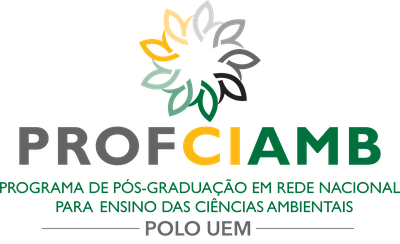
\includegraphics[width = 2cm]{logo.png}} %
       node at ([xshift=2cm,yshift=-2cm] current page.north west)
            {
\includegraphics[width = 2cm]{uem.png}}; %<- change the name of image
     \end{tikzpicture}}
}

% ---
% Configurações do pacote backref
% Usado sem a opção hyperpageref de backref
\renewcommand{\backrefpagesname}{Citado na(s) página(s):~}
% Texto padrão antes do número das páginas
\renewcommand{\backref}{}
% Define os textos da citação
\renewcommand*{\backrefalt}[4]{
   \ifcase #1 %
      Nenhuma citação no texto.%
   \or
      Citado na página #2.%
   \else
      Citado #1 vezes nas páginas #2.%
   \fi}%
% ---

% --- Informações de dados para CAPA e FOLHA DE ROSTO ---
\titulo{Representações sociais da poluição nas práticas de ensino: \\ Estado do conhecimento \\}

\tituloestrangeiro{\vspace{10 mm}  \normalsize{\textbf{Área Temática:} Representações sociais da poluição}}

\autor{Prof. Dr. Carlos Alberto de Oliveira Magalhães Júnior \\ email \href{juniormagalhaes@hotmail.com}{juniormagalhaes@hotmail.com} 
   \and Mestrando João Henrique da Silva \\ email \href{000jhs@gmail.com}{000jhs@gmail.com}}

\data{Departamento de Ciências - DCI -- Universidade Estadual de Maringá - UEM \\
        Maringá -- PR -- Brasil \\ Novembro - 2022}
% ---

% ---
% Configurações de aparência do PDF final

% alterando o aspecto da cor azul
\definecolor{blue}{RGB}{41,5,195}

% informações do PDF
\makeatletter
\hypersetup{
      %pagebackref=true,
      pdftitle={\@title}, 
      pdfauthor={\@author},
      pdfsubject={Estado do conhecimento - Representações sociais},
       pdfcreator={João Henrique da Silva},
      pdfkeywords={Representações sociais}{Poluição}{Novo Ensino Médio}, 
      colorlinks=true,           % false: boxed links; true: colored links
      linkcolor=blue,            % color of internal links
      citecolor=blue,            % color of links to bibliography
      filecolor=magenta,            % color of file links
      urlcolor=blue,
      bookmarksdepth=4
}
\makeatother
% --- 

% ---
% compila o indice
% ---
\makeindex
% ---

% ---
% Altera as margens padrões
% ---
\setlrmarginsandblock{3cm}{3cm}{*}
\setulmarginsandblock{3cm}{3cm}{*}
\checkandfixthelayout
% ---

% --- 
% Espaçamentos entre linhas e parágrafos 
% --- 

% O tamanho do parágrafo é dado por:
\setlength{\parindent}{1.3cm}

% Controle do espaçamento entre um parágrafo e outro:
\setlength{\parskip}{0.2cm}  % tente também \onelineskip

% Espaçamento simples
\SingleSpacing


% ----
% Início do documento
% ----
\begin{document}

% Seleciona o idioma do documento (conforme pacotes do babel)
%\selectlanguage{english}
\selectlanguage{brazil}

% Retira espaço extra obsoleto entre as frases.
\frenchspacing 

% ----------------------------------------------------------
% ELEMENTOS PRÉ-TEXTUAIS
% ----------------------------------------------------------

%---
%
% Se desejar escrever o artigo em duas colunas, descomente a linha abaixo
% e a linha com o texto ``FIM DE ARTIGO EM DUAS COLUNAS''.
% \twocolumn[        % INICIO DE ARTIGO EM DUAS COLUNAS
%
%---

% página de titulo principal (obrigatório)
\maketitle


% titulo em outro idioma (opcional)



% resumo em português
\begin{resumoumacoluna}
   O presente artigo se insere no contexto das pesquisas sobre representações sociais.
   Observa-se a lacuna nos estudos das representações sociais existente no ensino de ciências ambientais.
   Pretende-se levantar os dados acerca da referida produção acadêmica presente segundo a CAPES.
   Utiliza-se de ferramentas quantitativas e qualitativas para avaliar o estado do conhecimento na referida base de dados.
   Percebe-se uma vasta produção acerca do tema e apresenta-se um fluxo de trabalho para a filtragem e seleção das obras, com base na ocorrência de termos chave relevantes.
   Conclui-se que a a produção científica acerca do tema e dentro do recorte proposto se encontra amadurecida e destaca-se o caráter quantitativo e transdisciplinar desta. 

 \vspace{\onelineskip}
 
 \noindent
 \textbf{Palavras-chave}: Representações sociais. Poluição. Novo Ensino Médio.
\end{resumoumacoluna}


% ----------------------------------------------------------
% ELEMENTOS TEXTUAIS
% ----------------------------------------------------------
\textual

% ----------------------------------------------------------
% Introdução
% ----------------------------------------------------------
\section{Introdução}

O presente documento traz uma análise do estado do conhecimento na produção científica que emprega as representações sociais da poluição, considerando as produções científicas realizadas até o ano de 2021. Percebe-se como a metodologia das representações, desenvolvida por \citeonline{Representacees_sociais_moscovici} se encontra difundida nos  diversos campos do conhecimento e foca-se especificamente no escopo dos estudos realizados sobre o Novo Ensino Médio e, finalmente, discute-se seus resultados e possíveis aplicações. Para tanto utiliza-se os registros de textos monográficos, teses de doutorado e dissertações de mestrados presentes no catálogo de Teses e Dissertações da \citeonline{catalogo_capes}. 

% ----------------------------------------------------------
% Seção de explicações
% ----------------------------------------------------------
\section{Metodologia}

Para se realizar o presente levantamento, utilizou-se de um script original \cite{Python_NLTK_capes}, desenvolvido para esta exploração, com base nas ferramentas presentes na linguagem da programação Python para automação de raspagem de dados \cite{python_selenium} e subsequente análise linguística computacional \cite{Python_NLTK} visando a comparação dos conteúdos obtidos. Partindo dos dados coletados, foram definidos os agregados apresentados e selecionada a fração mais relevante da produção corrente na área para análise aprofundada. Na primeira seção apresenta-se uma descrição quantitativa da produção corrente. Segue-se daí uma descrição qualitativa dos conteúdos considerados relevantes.


\section{Resultados e discussões}

\subsection{Representações sociais no ano de 2021}

O aproveitamento da metodologia das representações sociais para a produção intelectual no nível de pós graduação, no contexto do Brasil, têm se mantido estável, se considerarmos o quantitativo anual indexado no catálogo de Teses e Dissertações da \citeonline{catalogo_capes}. Percebe-se uma ligeira retração do quantitativa da produção no ano de 2020, fato que pode estar relacionado com o período agudo da epidemia de Covid-19.

\begin{table}[htb]
\centering
\caption{Produção científica acerca das representações sociais por ano.}
\label{tab-nivinv}
\begin{tabular}{p{6.0cm}|p{6.0cm}}
  %\hline
    \textbf{Ano} & \textbf{Quantitativo} \\
    \hline
    2017 & 18221 \\
    \hline
    2018 & 19290 \\
    \hline
    2019 & 20265 \\
    \hline
    2020 & 17860 \\
    \hline
    2021 & 18229 \\
    \hline
    \hline
    Total & 93865 \\
\end{tabular}
\legend{Fonte: \citeonline{catalogo_capes}}
\end{table}

Encontra-se no banco de dados da \citeonline{catalogo_capes}, a quantidade de 18229 resultados para a busca do termo 'representações sociais' referentes ao ano de 2021. O quantitativo da produção pode ser subdividido considerando-se as modalidades de pós-graduação como demonstrado na tabela seguinte.

\begin{table}[htb]
\centering
\caption{Distribuição da produção acerca das representações sociais em 2021.}
\label{tab-nivinv}
\begin{tabular}{p{6.0cm}|p{6.0cm}}
  %\hline
   \textbf{Modalidade da Produção} & \textbf{Quantitativo} \\
    \hline
    Doutorado & 3841 \\
    \hline
    Doutorado profissional & 4 \\
    \hline
    Mestrado & 10542 \\
    \hline
    Mestrado profissional & 3842 \\
    \hline
    \hline
    Total & 18229 \\
\end{tabular}
\legend{Fonte: \citeonline{catalogo_capes}}
\end{table}


Percebe-se que a metodologia é aproveitada por estudos em diversas áreas e que as variações da aplicação da metodologia respondem às especifidades dos diversos objetos estudados. Destaca-se a produção na grande área das ciências sociais aplicadas, seguido da grande área de pesquisa multidisciplinar.

\begin{table}[htb]
\centering
\caption{Distribuição das grandes áreas da produção acerca das representações sociais em 2021.}
\label{tab-nivinv}
\begin{tabular}{p{6.0cm}|p{6.0cm}}
  %\hline
   \textbf{Grande área da produção} & \textbf{Quantitativo} \\
    \hline
    Ciências agrárias & 40 \\
    \hline
    Ciências biológicas & 20 \\
    \hline
    Ciências da saúde & 393 \\
    \hline
    Ciências exatas e da terra & 68 \\
    \hline
    Ciências humanas & 2119 \\
    \hline
    Ciências sociais aplicadas & 12024 \\
    \hline
    Engenharias & 38 \\
    \hline
    Lingüística, letras e artes & 722 \\
    \hline
    Multidisciplinar & 2805 \\
    \hline
    \hline
    Total & 18229
\end{tabular}
\legend{Fonte: \citeonline{catalogo_capes}}
\end{table}

\begin{figure}
   \caption{Distribuição das grandes áreas da produção acerca das representações sociais em 2021.}
   \begin{center}
       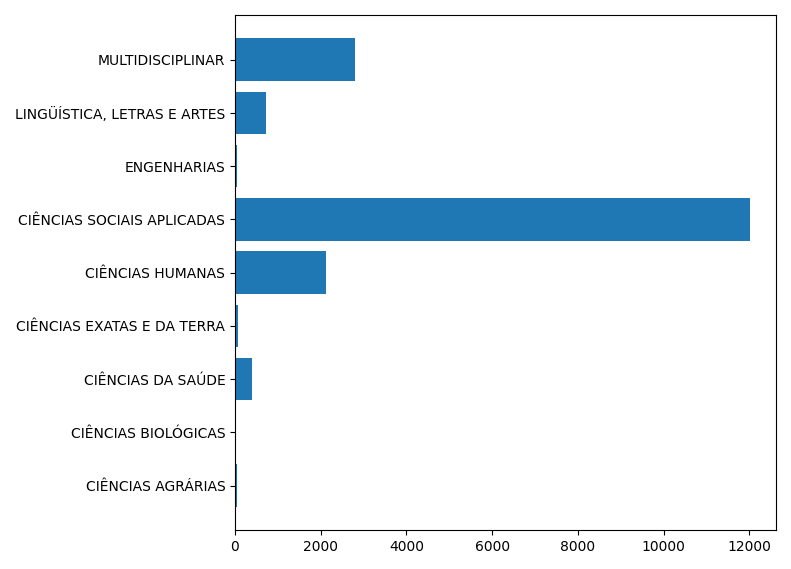
\includegraphics[width=120mm,scale=1]{est_con_2021.png}
   \end{center}
   \legend{Fonte: \citeonline{catalogo_capes}}
\end{figure}


\subsection{Representações sociais no ensino ensino ambiental}

O quantitativo de resultados retornado pelo referido banco de dados ao se expandir o escopo da pesquisa proposta para contemplar os quatro seguintes termos-chave 'representações sociais ensino ensino ambiental' surpreende pela abrangência, ao totalizar 480821 publicações. Tal aumento no quantitativo de resultados frente ao escopo limitado ao termo 'representações sociais', com 93865 registros indica particularidades do funcionamento do mecanismo de busca\footnote{O mecanismo de busca presente no referido banco de dados não apresenta de maneira clara os critérios do processamento do input do usuário. Portanto, não fica claro se uma concatenação de termos e.g. 'representações + sociais' é entendida pelo mecanismo de busca como o agregado de todas as ocorrências para o termo 'representações' associado ao agregado de todas as ocorrências para o termo 'sociais'. Esta primeira impressão parece válida, visto que o destaque dado para a concatenação de termos 'representações + sociais', enquanto unidade semântica, aparece para o usuário misturada às ocorrências isoladas de cada termo. Tal fator pode enviesar as interpretações dos resultados visto que, um primeiro termo concatenado com um segundo pode inflar o quantitativo dos resultados e causar uma falsa impressão de relevância. Tal impressão pode sedar pelo fato de o mecanismo de busca considerar os conteúdos dos registros no banco de dados através de um escopo que vai além dos conteúdo apresentados para o usuário. Nesta situação, os dados da concatenação de termos pesquisada seriam críveis visto que os resultados apresentados ao usuário seriam sintomáticos de informações obscurecidas. A relevância de tal observação se mostra ao se concatenar mais que dois termos, e.g. 'representações + sociais + poluição', situação que retorna um número maior de resultados, 315857, frente os 308196 resultados retornados para a concatenação de termos 'representações + sociais'. Sugere-se que a inserção de uma quantidade maior de termos deveria retornar uma quantidade menor de resultados visto que a probabilidade de se atender a um número maior de condicionantes deveria reduzir, e não aumentar, a quantidade de resultados. Conclui-se daí que todas as combinações possíveis entre os três termos devem estar sendo requisitadas, fato que pode incluir falsos positivos como aqueles oriundos da combinação entre os termos 'representações' + 'poluição' desassociados ao termo 'social', trazendo para o usuário informações as quais podem ser sintomáticas de discussões alheias àqueles requisitados nas pesquisas com mais de dois termos.} no portal da capes que serão discutidas adiante. Visando estreitar o escopo, pode-se restringir o período temporal para selecionar apenas a produção no ano de 2021, observando-se apenas as produções de Doutorado (89101 publicações), Doutorado Profissional (13 publicações), Mestrado (318970 publicações), Mestrado Profissional (61297 publicações), totalizando 469381 publicações, das quais foram produzidas em 2021, nos níveis de Doutorado (6004 publicações), Doutorado Profissional (5 publicações), Mestrado (15843 publicações) e Mestrado Profissional (8377 publicações), totalizando 30229 publicações.

Interessa aqui estreitar a ainda mais a análise afim de se perceber como se situa a produção no interior das grandes áreas do conhecimento. Para tanto, os dados obtidos nos informam que dentro das grades áreas das Ciências sociais aplicadas e da pesquisa multidisciplinar, a produção totaliza 14829 publicações e se divide nas seguintes 45 áreas listadas na tabela 4, em anexo. Decorre daí que o recorte mais relevante para a pesquisa aqui proposta inclui a produção na frande área do conhecimento multidisciplinar, com 7350 publicações onde encontra-se a área as ciências ambientais com 992 publicações, a qual contempla a área de concentração do ensino de ciências ambientais, na qual encontra-se 105 publicações, as quais convergem qualitativamente com o recorte aqui proposto. Este recorte entrega um quantitativo acessível que permite a subsequente análise qualitativa, e os resultados apresentados adiante foram obtidos usando o script para automação de raspagem de dados \cite{python_selenium} e subsequente análise linguística computacional \cite{Python_NLTK} presente no segundo anexo.

Dentro dos resumos das 105 publicações selecionadas, encontra-se a terminologia que interessa à pesquisa proposta ao se identificar a ocorrência e coocorrência de quatro termos específicos, sendo estes, em ordem de prioridade: 'representações', 'sociais', 'ensino' e 'poluição', os quais foram identificados no material selecionado através da busca por seus respectivos elementos radicais, i.e. 'represent', 'soc', 'ensin' e 'polu'. Pode-se ilustrar as associações entre os termos isolados e sua relevância usando do diagrama de Reinert, técnica a qual permite inferências entre as coocorrências de termos no conjunto dos resumos. 

\begin{figure}
   \caption{Distribuição de Reinert grandes áreas da produção acerca das representações sociais em 2021.}
   \begin{center}
       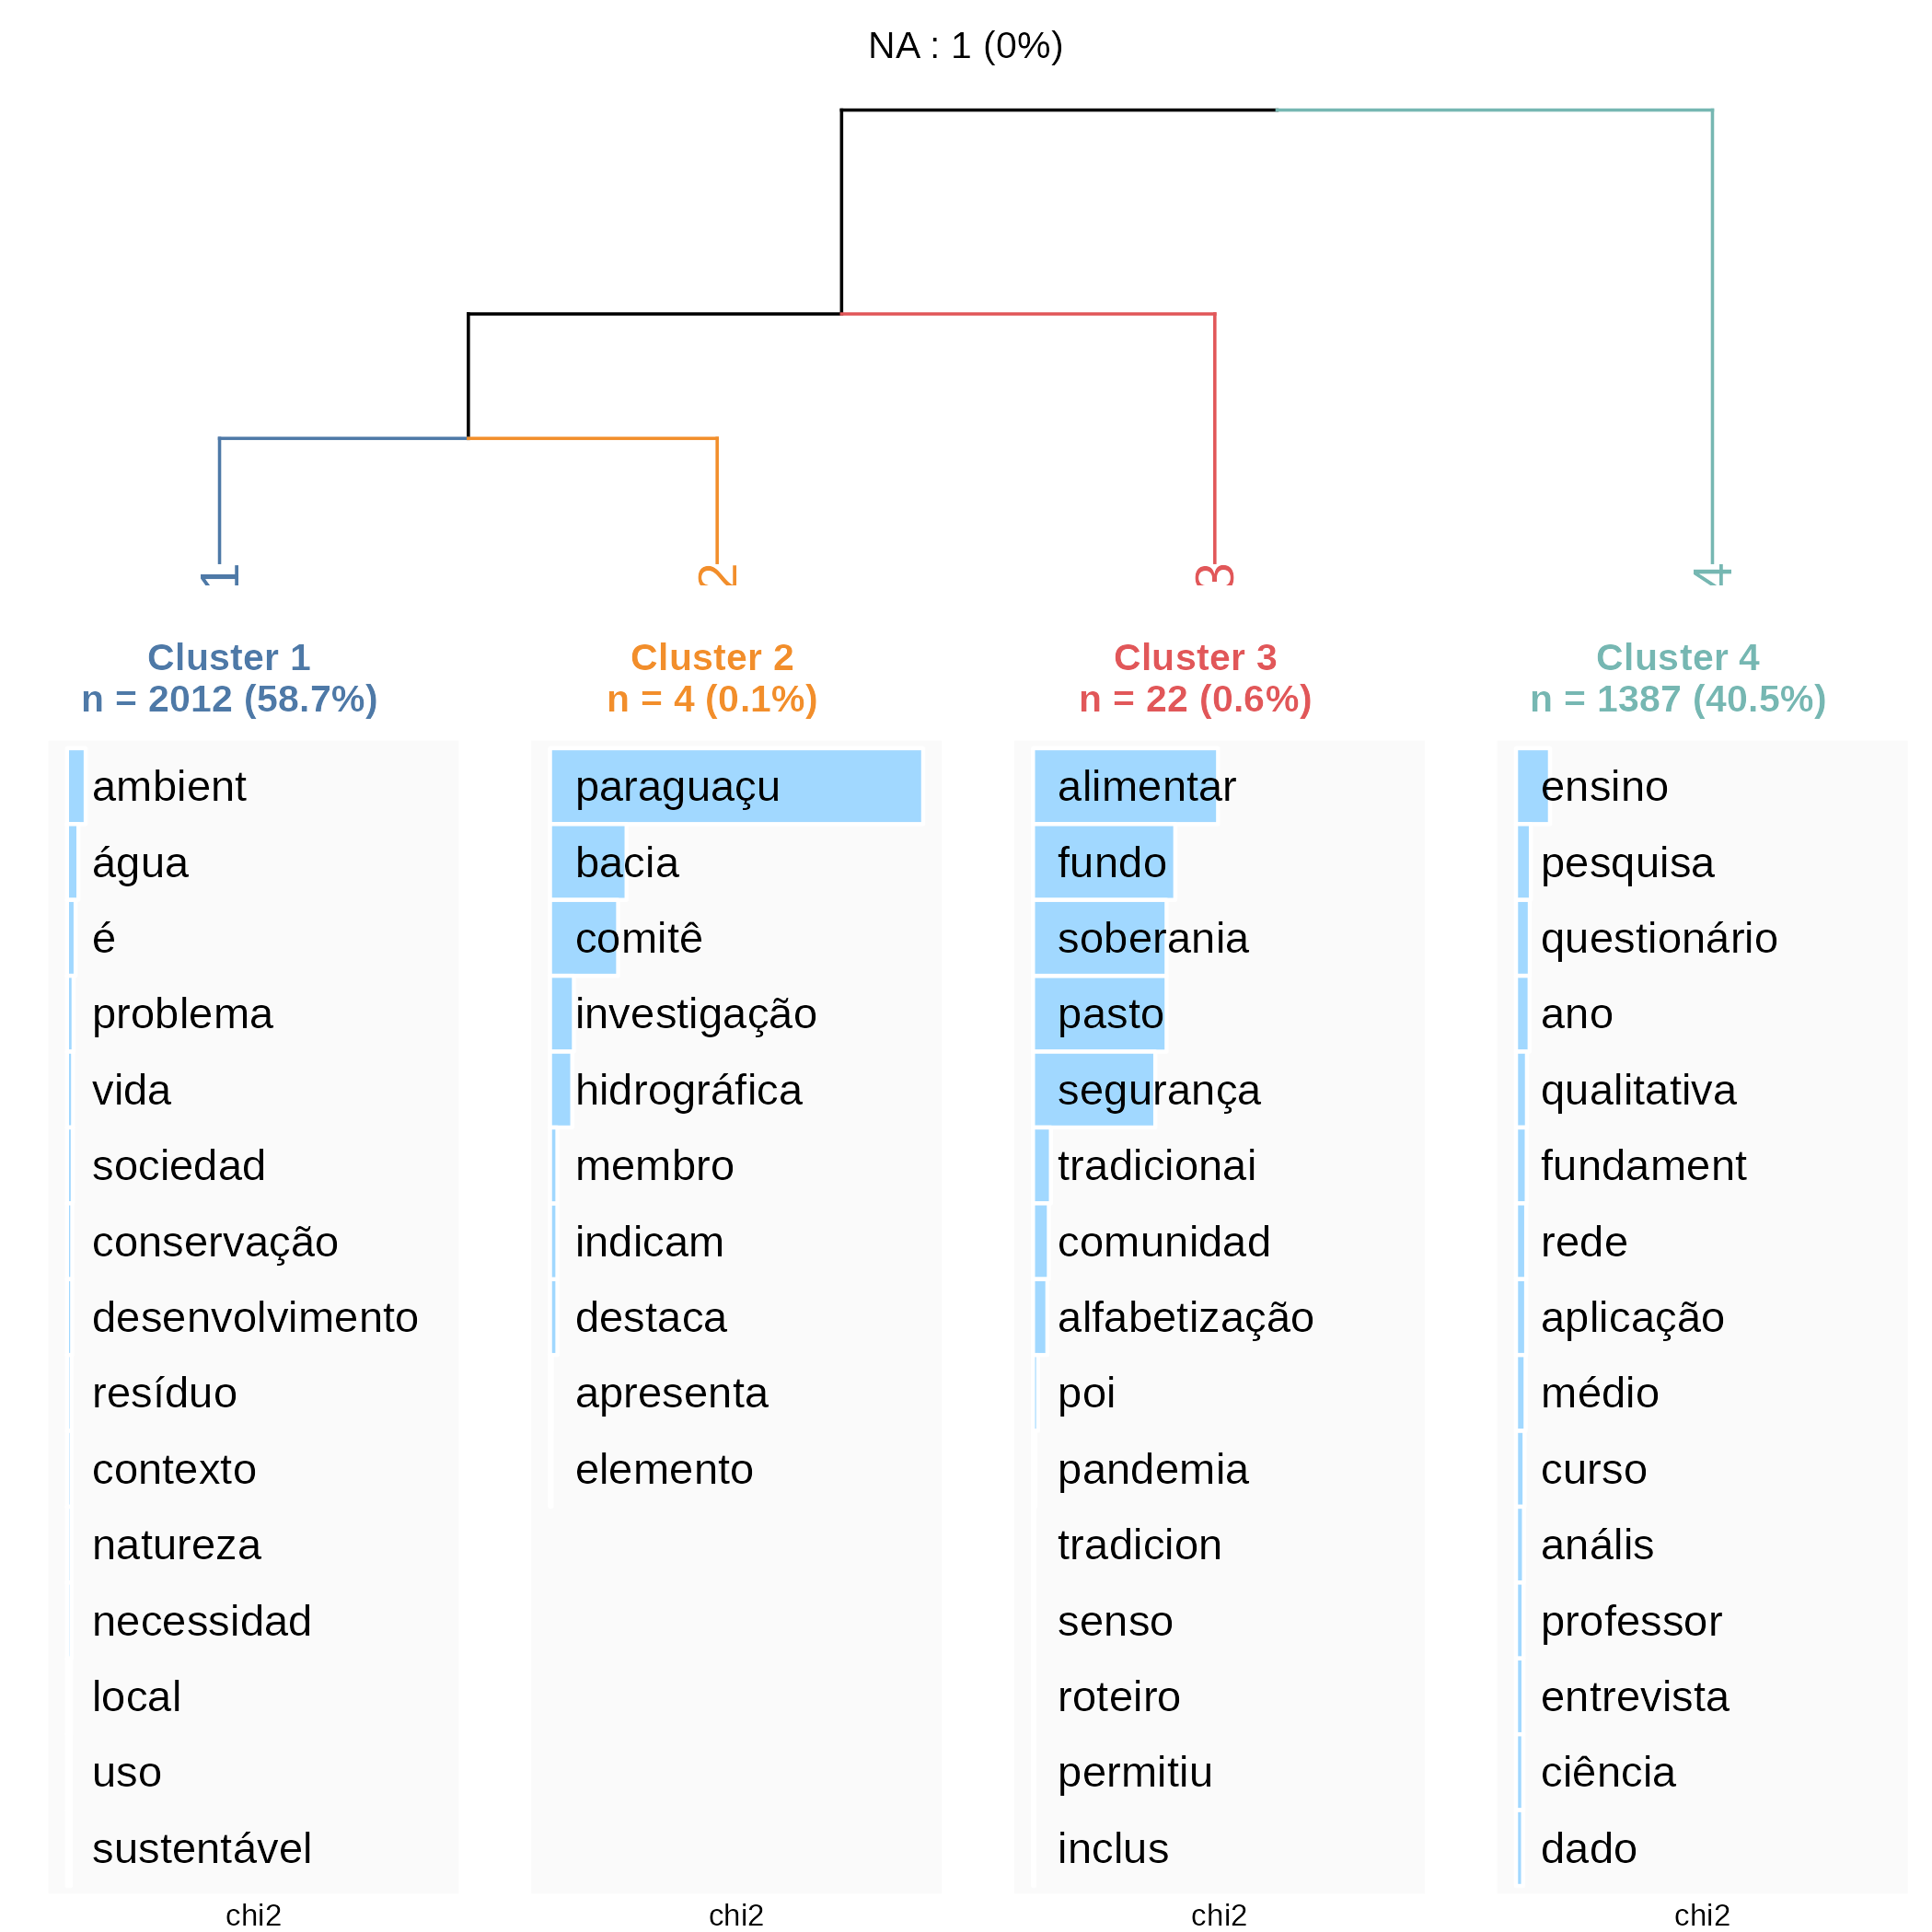
\includegraphics[width=120mm,scale=1]{resumes_reinert.png}
   \end{center}
   \legend{Fonte: Elaborado pelo autor.}
\end{figure}

\subsection{Representações e ensino}
O termo representações aparece isolado nos resumos em apenas 9 das publicações selecionadas; percebe-se daí que a presença do termo, verificada usando o radical, coocorre junto ao termo ensino e se apresenta em 15 trabalhos, dentro dos selecionados.
Quando se soma aos termos 'representações' e 'ensino', a terceira categoria 'sociais' afim de denotar a convergência proposta pelo recorte adotado, a quantidade de trabalhos cujos resumos carregam tais temas se expande para 19 obras.


\subsubsection{Representações da poluição segundo discentes do ensino fundamental}
O recorte pode ser expandido para incluir outros elementos relevantes. Ao se considerar a coocorrência do termo fundamental, denotado pelo radical 'fundament', expande-se o escopo dos trabalhos e encontra-se 29 obras cujos resumos carregam tais temas. Ao se incluir o objeto 'poluição' denotado pelo radical 'polu', a quantidade de trabalhos cujos resumos carregam tais temas se expande para 34 obras. 


\subsubsection{Representações segundo discentes do Novo Ensino Médio}
O tema do Novo Ensino Médio, não foi encontrado nos resumos selecionados, situação que indica a necessidade de se realizarem estudos originais, dentro deste recorte da educação contemporânea.


\subsubsection{Representações da poluição e geração de energia}
Ao se expandir o tema e incorporar outros elementos, percebe-se que o escopo das obras ilustra a capilaridade e o caráter interdisciplinar das investigações. O termo energia, denotado pelo radical 'energ' coocorre com os termos 'representações', 'ensino', 'poluição' gerando um conjunto de 26 obras cujos resumos abordam tais objetos.

\subsubsection{Representações da poluição, consumo e lixo}
O agregado mais amplo apresentado aqui incorpora os termos acima apresentados e soma os termos 'fundamental' 'indústria' e 'lixo', denotados pelos respectivos radicais
'fundament', 'indústr', 'lix', gerando um conjunto de 52 obras cujos resumos apresentam tais termos.


\section{Considerações finais}

Percebe-se que o escopo da terminologia usada nas palavras-chave da pesquisa proposta permeia diversas áreas do conhecimento. Destaca-se aí o caráter interdisciplinar das propostas em educação ambiental, característica que exigem a filtragem dos resultados apresentados pelo referido portal. A seleção de obras no banco de dados da Capes deve ser então seguida de um processo de filtragem similar ao processo aqui apresentado, o qual permita perceber e selecionar grupos de obras as quais compartilhem temas e métodos. Acerca especificamente do tema das representações sociais, este se apresenta difundido em diversas áreas do conhecimento, com especial destaque para as áreas de ciências sociais aplicadas, multidisciplinar, e da linguística. A aplicação de tal metodologia nos estudos da educação está contemplada, de maneira implícita, nestes três recortes. A ausência de estudos de estudos de representações sociais no contexto do Novo Ensino Médio é um fato de destaque, dado pela novidade do formato de ensino em questão.


\bibliography{Interdisciplinaridade}

% Imprime uma página indicando o início dos anexos
\partanexos

\begin{table}[htb]
\centering
\caption{Distribuição das áreas da produção acerca das representações sociais em 2021.}
\label{tab-nivinv}
\begin{tabular}{p{8.0cm}|p{4.0cm}}
   \textbf{Área da produção} & \textbf{Quantitativo} \\
   \hline
   Administração  &  1944 \\
   \hline
   Administração de empresas  &  459 \\
   \hline
   Administração de setores específicos  &  20 \\
   \hline
   Administração pública  &  478 \\
   \hline
   Arquitetura e urbanismo  &  668 \\
   \hline
   Arquivologia  &  1 \\
   \hline
   Biblioteconomia  &  18 \\
   \hline
   Ciência da informação  &  406 \\
   \hline
   Ciências ambientais  &  46 \\
   \hline
   Ciências contábeis  &  377 \\
   \hline
   Comunicação  &  918 \\
   \hline
   Comunicação visual  &  14 \\
   \hline
   Demografia  &  47 \\
   \hline
   Desenho industrial  &  335 \\
   \hline
   Direito  &  3182 \\
   \hline
   Direito constitucional  &  122 \\
   \hline
   Direito processual civil  &  1 \\
   \hline
   Direito público  &  210 \\
   \hline
   Direitos especiais  &  127 \\
   \hline
   Economia  &  984 \\
   \hline
   Economia agrária  &  40 \\
   \hline
   Economia dos recursos humanos  &  18 \\
   \hline
   Economia geral  &  11 \\
   \hline
   Economia regional  &  17 \\
   \hline
   Engenharia, tecnologia, gestão  &  27 \\
   \hline
   Ensino  &  127 \\
   \hline
   Ensino de ciências e matemática  &  78 \\
   \hline
   Finanças públicas internas  &  13 \\
   \hline
   Fundamentos do serviço social  &  41 \\
   \hline
   História do direito  &  30 \\
   \hline
   Interdisciplinar  &  4 \\
   \hline
   Jornalismo e editoração  &  11 \\
   \hline
   Meio ambiente e agrárias  &  48 \\
   \hline
   Mercadologia  &  23 \\
   \hline
   Museologia  &  56 \\
   \hline
   Negócios internacionais  &  28 \\
   \hline
   Planejamento urbano e regional  &  613 \\
   \hline
   Saúde e biológicas  &  80 \\
   \hline
   Serviço social  &  481 \\
   \hline
   Serviço social aplicado  &  78 \\
   \hline
   Sociais e humanidades  &  2395 \\
   \hline
   Tecnologia de arquitetura e urbanismo  &  24 \\
   \hline
   Teoria do direito  &  27 \\
   \hline
   Teoria econômica  &  66 \\
   \hline
   Turismo  &  136 \\
   \hline
   \hline
   Total  &  14829 \\

\end{tabular}
\legend{Fonte: \citeonline{catalogo_capes}}
\end{table}


\end{document}
